\section{Empirical Results}
\label{sec:results}

In this section we evaluate our novel SDP solution technique on three
domains: (1) continuous stochastic matching pennies; (2) continuous
binary option valuation; and (3) continuous energy production. 
The domain descriptions and results are presented
below.

\subsection{Continuous Stochastic Matching Pennies}

Matching pennies is a well known zero-sum game with a 
mixed Nash Equilibrium \cite{Osborne_2004}. In this paper we extend 
the standard formulation of the game by incorporating continuous state 
and sequential decisions while still maintaining the zero-sum nature of 
the reward.

\subsubsection{Domain Description}

We define continuous stochastic matching pennies as an extensive
form game between two players $p \in \left\{1, 2 \right\}$. The aim of a 
player is to maximise its expected discounted pay-off at a fixed horizon \emph{H}. 
Our game is played within the interval $[0, 1]$, two fixed variables 
$c \in [0, 1)$ and $d \in (0, 1]$ with $(c < d)$,  are used to partition the interval into
three regions $r \in \left\{1, 2, 3 \right\}$. Each region is associated 
with its own zero-sum reward structure. The continuous state variable 
$x \in [0, 1]$ is used to specify which region the the players are competing within.

At each horizon $(h \leq H)$ each player executes an action $a_p \in \left\{ heads_p, tails_p \right\}$. 
Player 1 ``wins'' if both players choose the same action. Otherwise, Player 2 wins. 
The joint actions of the players affect the state $x$ as follows:

{\small 
\abovedisplayskip=0pt
\belowdisplayskip=0pt
\begin{align*}
&P(x' | x, a_{1}, a_{2}) = \\
\\
& \hspace{10pt} \delta \left[ x' - \begin{cases}
      (heads_{1}) \wedge (heads_{2}) \wedge (x \geq k) : & x - k \\
      (heads_{1}) \wedge (tails_{2}) \wedge (x \leq 1) : & x + k \\
      (tails_{1}) \wedge (heads_{2}) \wedge (x \geq k): & x + k \\
      (tails_{1}) \wedge (tails_{2}) \wedge (x \leq 1) : & x - k  \\
    \end{cases} \right]
\end{align*}
}%

The constant $k \in (0, 1)$ is a step size which perturbs the state $x$. 
If Player 1 wins, the state moves to the left by $k$, otherwise it moves to the
right by $k$. The Dirac function $\delta[\cdot]$ ensures that the transitions are valid 
conditional probability functions that integrate to 1. We define the 
rewards obtained by Player 1 in region $r$ as:

{\small 
\abovedisplayskip=0pt
\belowdisplayskip=0pt
\begin{align}
\label{eq:cmpreward}
  R^r_{1} &= 
    \begin{cases}
     (heads_{1}) \wedge (heads_{2}) : & \alpha^{r}_{1} \\
     (heads_{1}) \wedge (tails_{2}) : & \alpha^{r}_{2} \\
     (tails_{1}) \wedge (heads_{2}) : & \alpha^{r}_{3} \\
     (tails_{1}) \wedge (tails_{2}) : & \alpha^{r}_{4} \\
    \end{cases}
\end{align}
}%

Here we restrict $\alpha^{r}_i \in \mathbb{R}$. The rewards obtained 
by Player 2 in the same region are simply $-R^r_{1} $. Henceforth, we
define rewards from the perspective of Player 1. Given this domain description, 
we investigate the affects of symmetric and asymmetric reward structures 
on the continuous stochastic matching pennies game. We define a 
symmetric reward structure as having $\alpha^{r}_1 = \alpha^{r}_4$ and 
$\alpha^{r}_2 = \alpha^{r}_3$. Under a symmetric reward structure
the expected reward in each region is the same for both players. An 
asymmetric reward structure allows the $\alpha^{r}_i$ to differ in both
sign and magnitude. Under this setting the expected rewards for a player may differ across
regions. Tables \ref{tab:smpsymreward} and \ref{tab:smpasymreward}
show examples of symmetric and asymmetric rewards for the 
continuous stochastic matching pennies domain.

\begin{table}[h!]
\caption{Symmetric reward structure for Player 1. Note that symmetric 
nature of the rewards within each region and the differing rewards between regions.}
\label{tab:smpsymreward}
\begin{tabular}{ l | c | c | c |}
\cline{2-4}   
  & Region 1 & Region 2 & Region 3 \\ \hline
  \multicolumn{1}{ |l| }{$(heads_{1}) \wedge (heads_{2})$} & 10 & 5 & 20 \\ \hline
  \multicolumn{1}{ |l| }{$(heads_{1}) \wedge (tails_{2})$} & -10 & -5 & -20 \\ \hline
  \multicolumn{1}{ |l| }{$(tails_{1}) \wedge (heads_{2})$} & -10 & -5 & -20 \\ \hline
  \multicolumn{1}{ |l| }{$(tails_{1}) \wedge (tails_{2})$}    & 10 & 5 & 20 \\  
  \hline
\end{tabular}
\end{table}

\begin{table}[h!]
\caption{Asymmetric reward structure for Player 1. Note that asymmetric 
nature of the rewards within each region and the differing rewards between regions.}
\label{tab:smpasymreward}
\begin{tabular}{ l | c | c | c |}
\cline{2-4}   
  & Region 1 & Region 2 & Region 3 \\ \hline
  \multicolumn{1}{ |l| }{$(heads_{1}) \wedge (heads_{2})$} & 1 & 5 & 7 \\ \hline
  \multicolumn{1}{ |l| }{$(heads_{1}) \wedge (tails_{2})$} & -3 & -5 & -2 \\ \hline
  \multicolumn{1}{ |l| }{$(tails_{1}) \wedge (heads_{2})$} & 0 & -5 & 10 \\ \hline
  \multicolumn{1}{ |l| }{$(tails_{1}) \wedge (tails_{2})$} & 2 & 5 & 20 \\  
  \hline
\end{tabular}
\end{table}

\subsubsection{Results}

%%%%%%%%%%%%%%%%%%%%%%%%%%%%%%%%%
% Figure
%%%%%%%%%%%%%%%%%%%%%%%%%%%%%%%%%

\begin{figure}[t!]
\vspace{-2mm}
\centering

\begin{subfigure}[b]{0.5\textwidth}
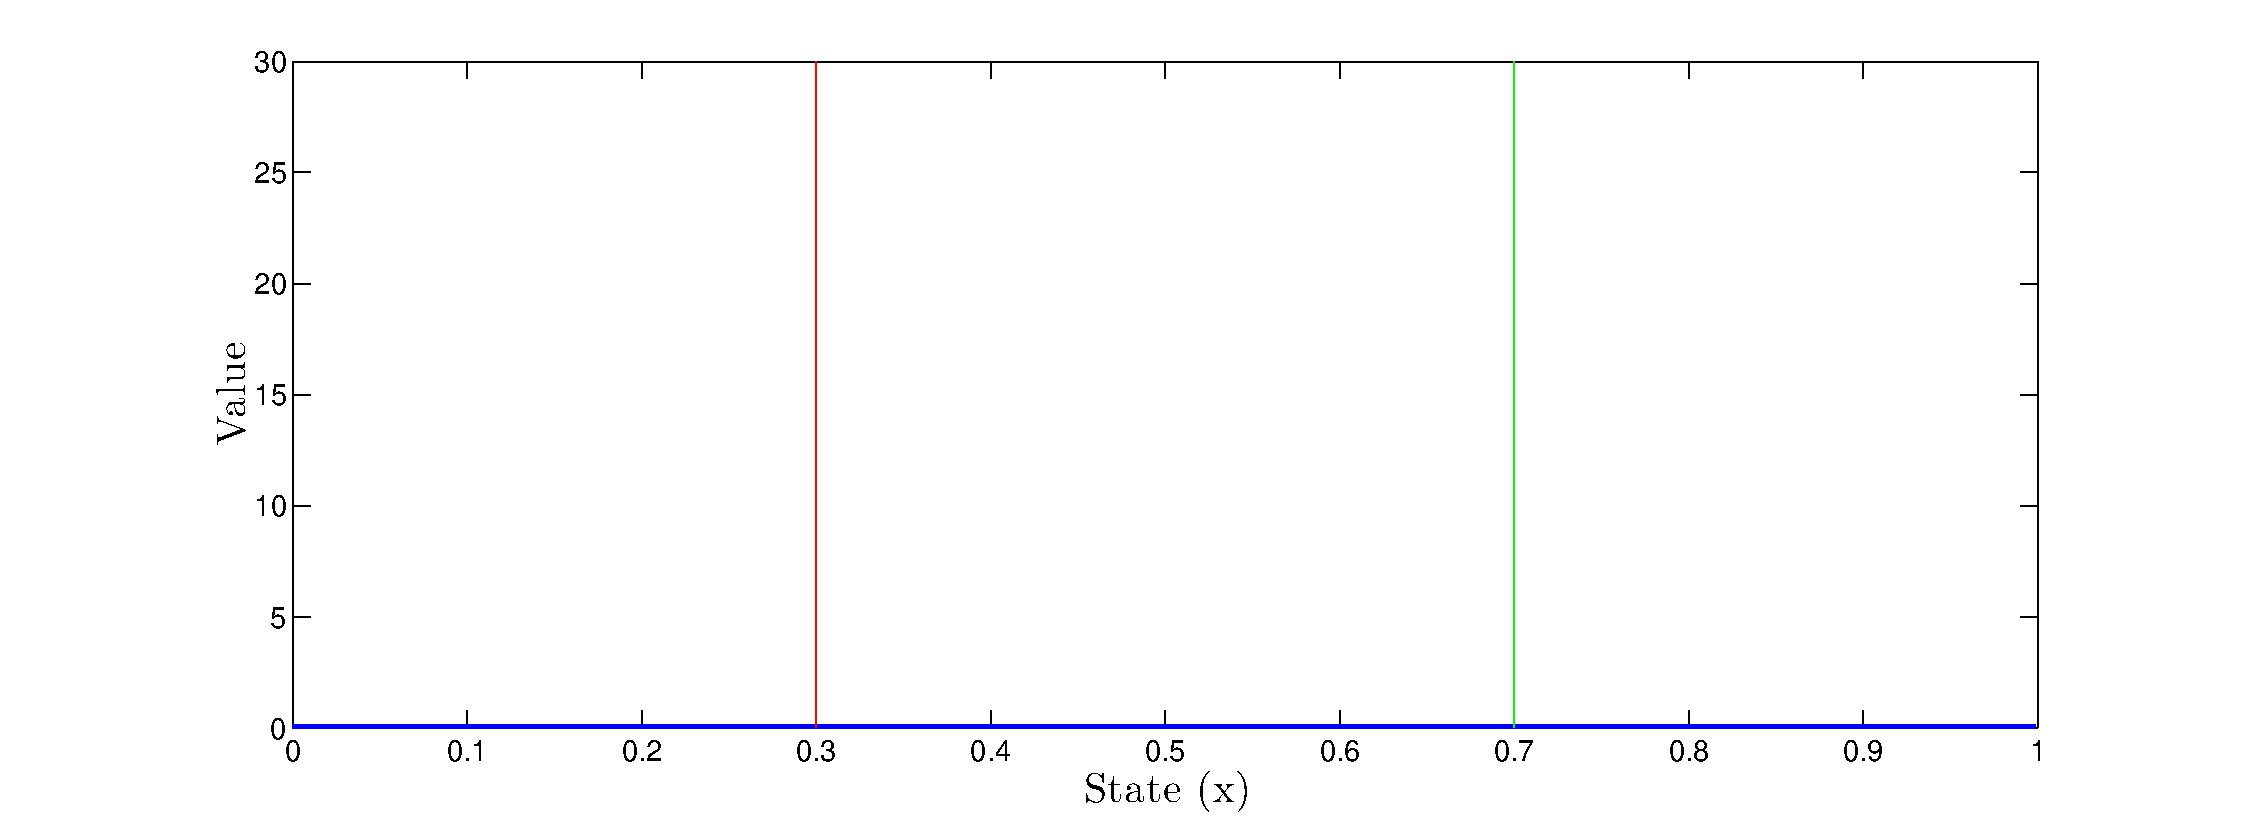
\includegraphics[width=260pt]{smp_sym.pdf}
\caption{Symmetric rewards.}
\label{fig:smpasmreward1}
\end{subfigure}

\begin{subfigure}[b]{0.5\textwidth}
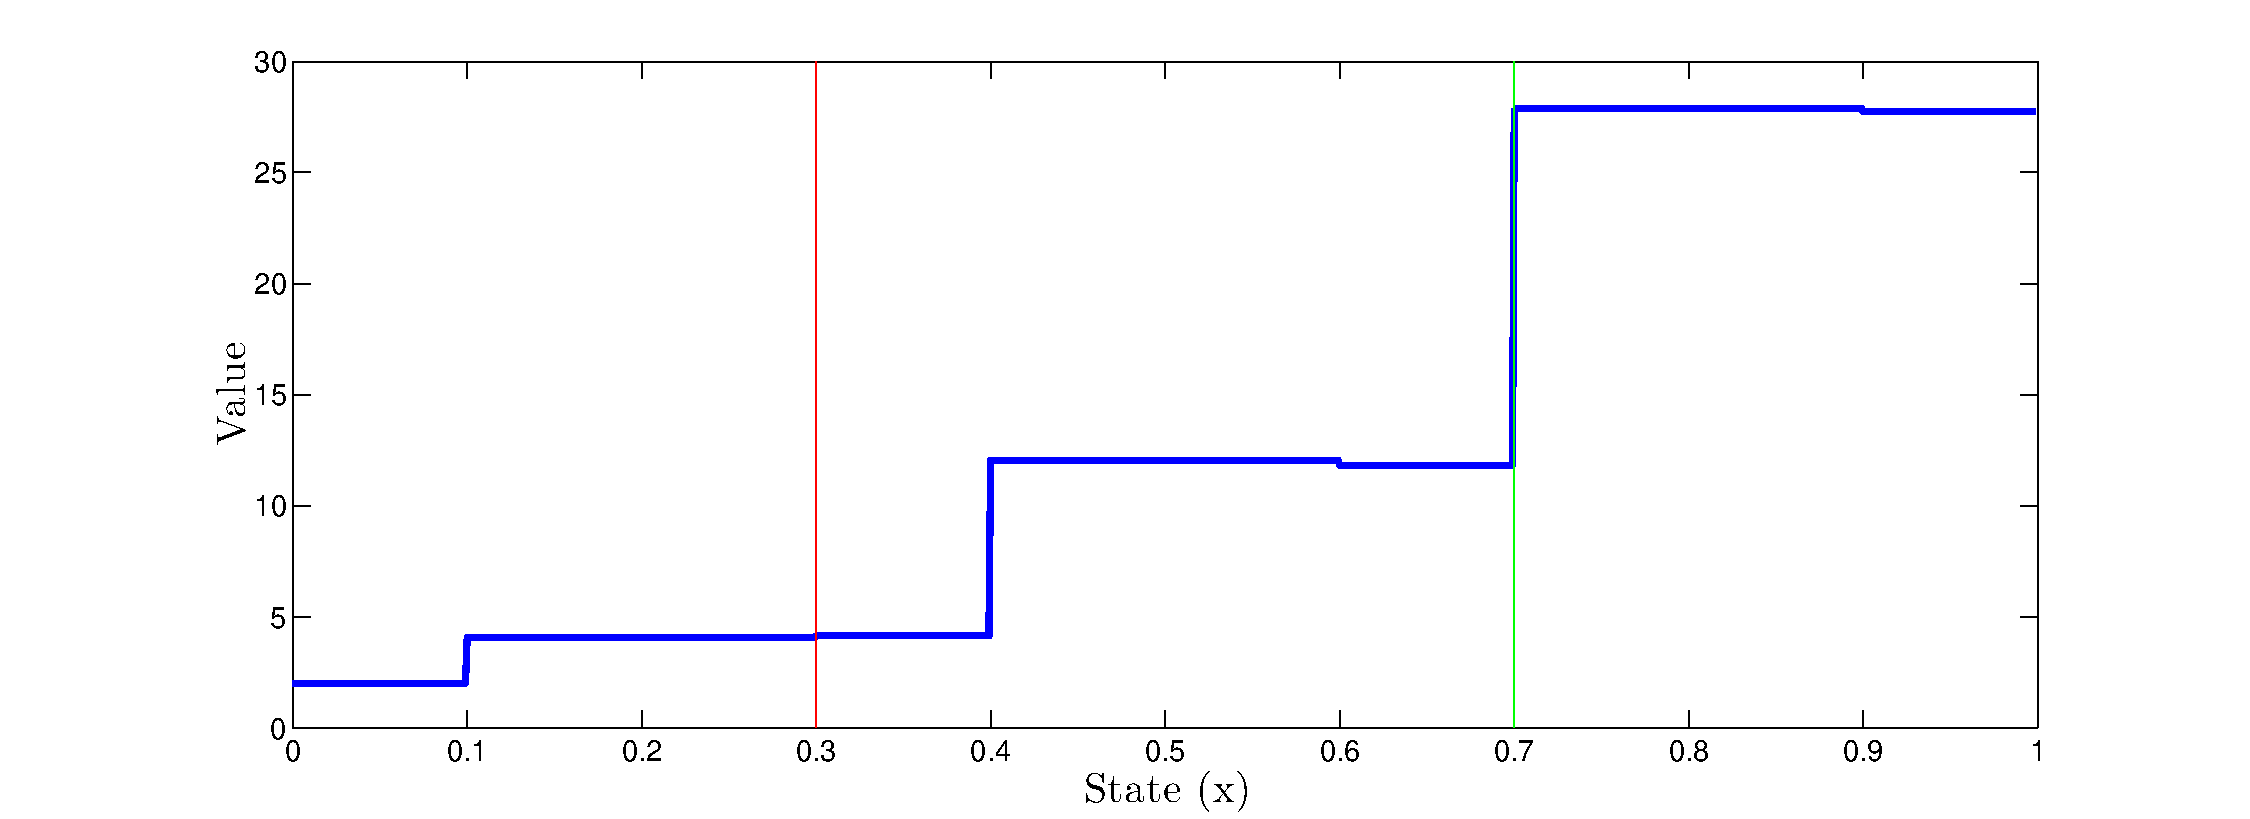
\includegraphics[width=260pt]{smp_asym.pdf}
\caption{Asymmetric rewards.}
\label{fig:smpasmreward2}
\end{subfigure}

\vspace{-2mm}
\caption{Optimal value functions for continuous stochastic matching 
            pennies under (a) symmetric and (b) asymmetric reward 
            structures at horizon 4. Threshold values $c$ 
            and $d$ are highlighted in red and green, respectively. 
            The step size is $k = 0.3$.}
\label{fig:smpasmreward}
\end{figure}

Figure \ref{fig:smpasmreward1} shows the results of the continuous
stochastic matching pennies game using the symmetric reward structure
given in Table \ref{tab:smpsymreward}. 
The results show that the expected reward for Player 1 remains at zero
over all 4 horizons, irrespective of the state $x$. Given the symmetric
rewards in each region, both players are indifferent between their 
pure strategies. Hence, the expected reward for each player is zero in
all regions. This corresponds to the well known solution of the 
matching pennies game where the rewards are symmetric and serves 
as a proof of concept for our novel solution technique.

The effect of the asymmetric reward structure, given in Table \ref{tab:smpasymreward}, 
is shown in Figure \ref{fig:smpasmreward2}. From the figure it is clear that Player 1 achieves the highest expected
reward in Region 3, followed by Region 2 and finally by Region 1. This
is to be expected given the nature of the asymmetric rewards within
each region. The results indicate that the two players are
no longer indifferent between their pure strategies in each region. 

\subsection{Binary Option Stochastic Game}

Binary options are financial instruments which allow an investor to
bet on the outcome of a yes/no proposition. The proposition typically
relates to whether the price of a particular asset that underlies the option
will rise above or fall below a specified amount, known as the strike
price, $\kappa \in \mathbb{R}$. When the option reaches maturity the 
investor receives a fixed pay-off if their bet was correct and nothing otherwise.

\subsubsection{Domain Description}

We analyse the valuation of a binary option as an extensive form
zero-sum game between a trader and the market. The aim of the trader
is to maximise their expected discounted pay-off at a fixed horizon $H$ 
through buying and selling options within an adversarial market. 
The problem has two state variables: the underlying market value of the option
$v \in [0, 100]$ and the trader's inventory of options $i \in \mathbb{N}$.

At each time step the trader can execute one of three actions
$a_{trd} \in \left\{buy_{trd}, sell_{trd}, hold_{trd}\right\}$, where $buy_{trd}$ refers to a request to 
buy an option from the market, $sell_{trd}$ refers to a request to sell an option to
the market and $hold_{trd}$ is equivalent to taking no action. 
The market can execute one of two actions: $a_{mkt} \in \left\{sell_{mkt}, nsell_{mkt} \right\}$,
where $sell_{mkt}$ corresponds to selling an option to the trader and $nsell_{mkt}$ 
corresponds to not selling to the trader. 

The joint actions of the trader and market, $a_{\text{trd}}$ and 
$a_{\text{mkt}}$, respectively, affect both the market value of the option
and the trader's inventory. For the sake of simplicity we assume that
the market value may increase or decrease by fixed step sizes, 
$u \in \mathbb{R}$ for an increase and $d \in \mathbb{R}$ for a decrease.

The trader's option inventory dynamics are given by:

{\small 
\abovedisplayshortskip=0pt
\belowdisplayshortskip=0pt
\begin{equation*}
P(i' | v, i, a_{\text{trd}}, a_{\text{mkt}}) = \delta \left[ i' - \begin{cases}
      (buy_{trd}) \wedge (sell_{mkt}) : & i + 1 \\ 
      (sell_{trd}) \wedge (i > 0) : & i - 1 \\
      otherwise: & i \\
    \end{cases} \right] \\
\end{equation*}
}%

It should be noted that under this formulation the market will always
buy an option from the trader when the trader selects $sell_{trd}$. 
The market value changes according to:

{\small 
\abovedisplayskip=0pt
\belowdisplayskip=0pt
\begin{align*}
P(v' | v, i, a_{\text{trd}}, a_{\text{mkt}}) &= \\
&
\delta \left[ v' - \begin{cases}
      (buy_{trd}) \wedge (sell_{mkt})  : & v + u \\
       (sell_{trd}) \wedge (i > 0) : & v - d \\
      otherwise: & v
    \end{cases} \right] & \\    
\end{align*}
}%

%The market value of the option is contingent upon the actions of the
%trader and a Bernoulli distributed random variable, $\epsilon \sim \text{Bernoulli}(p)$, 
%where $p \in [0, 1]$. By varying the parameter $p$ the latent market
%dynamics can be made to approximate a bull or bear market.

Assuming that the strike price $\kappa \in [0, 100]$, the rewards obtained by the trader are given by:
{\small 
\begin{equation}
  R_{trader} = 
    \begin{cases}
      (sell_{trd}) \wedge (i > 0) \wedge (v > \kappa) : & 1 \\ 
      otherwise : & 0 \\
    \end{cases} \nonumber
\end{equation}
}%

The market's reward is simply the additive inverse of the trader's 
reward. Hence, the binary option game is zero-sum. 

\subsubsection{Results}

%%%%%%%%%%%%%%%%%%%%%%%%%%%%%%%%%
% Figure
%%%%%%%%%%%%%%%%%%%%%%%%%%%%%%%%%

\begin{figure}[h!]
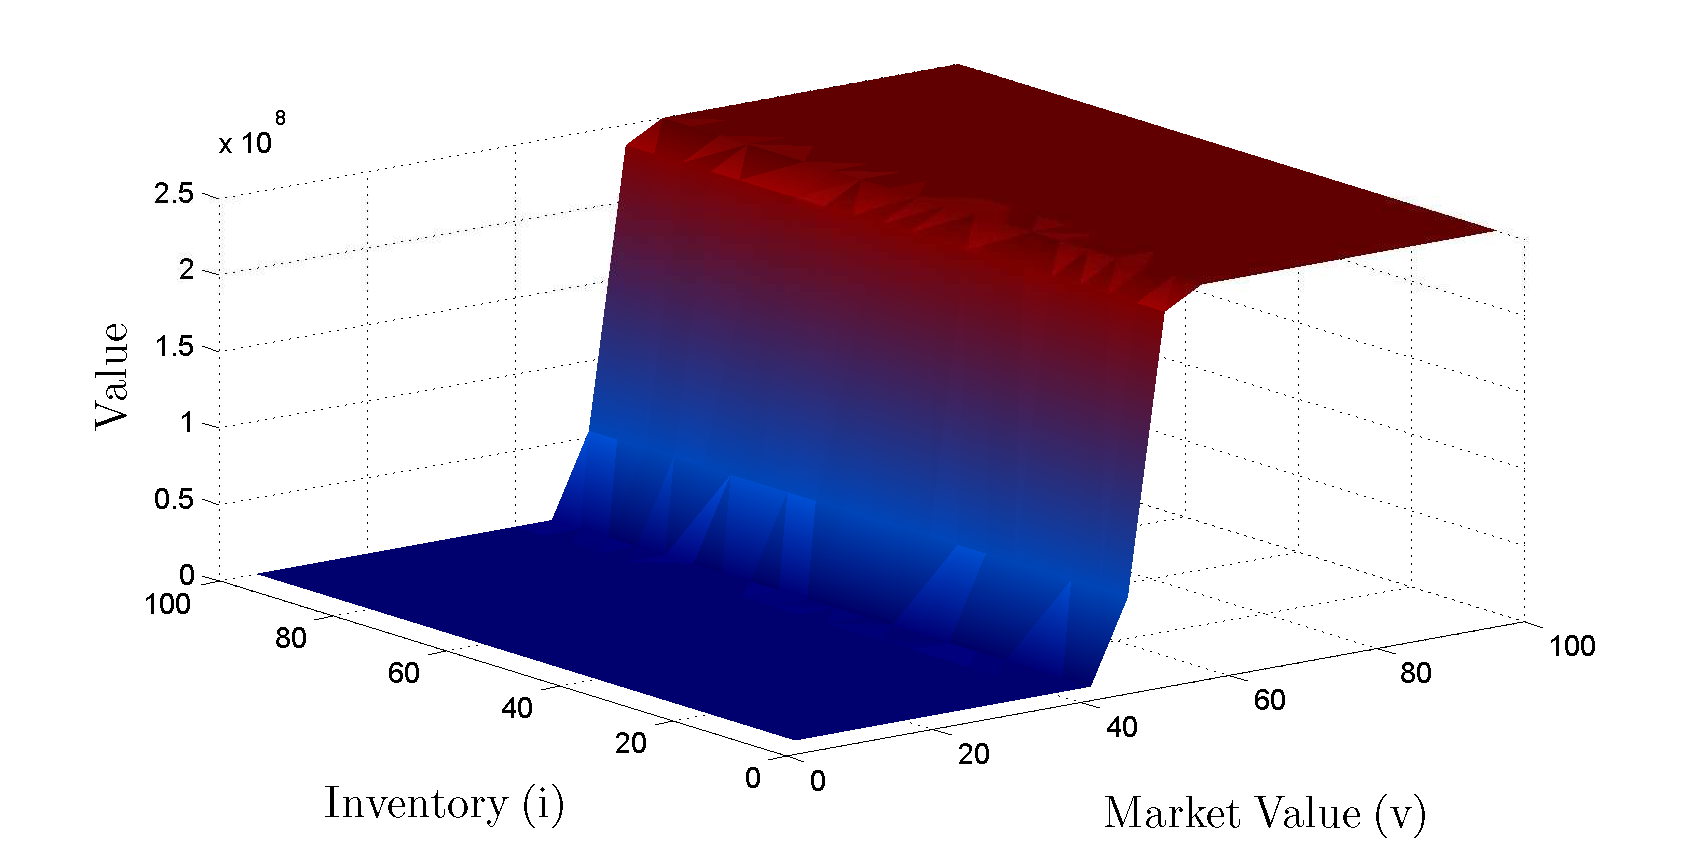
\includegraphics[width=250pt]{sbo.pdf}
\vspace{-3mm}
\caption{The optimal value function for the binary option game at horizon 20. The strike price is set to $\kappa = 45.0$ and the increment and
decrement values are set to $u = 1.0$ and $d = 1.0$, respectively.}
\label{fig:binaryoptionvfunc}
\end{figure}

In Figure \ref{fig:binaryoptionvfunc} we show the optimal value function for the
binary option game at horizon 20. The strike price $\kappa = 45.0$ and
the increment and decrement values, $u$ and $d$ are both set to 1.0. The
value function clearly shows that under this formulation the trader
achieves the most reward by selling the option as soon $v > \kappa$.
Selling an option triggers the underlying value to decrease, which triggers
the trader to buy once the value falls beneath the strike price. This leads
to the continual cycling of buying and selling of the option at values close
to the strike price $\kappa$. In essence the trader behaves like a market
maker in that they take both sides of the transaction at values near 
$\kappa$.

\subsection{Robust Energy Production}

The provision of energy resources is an integral component of any
economy. Energy providers must be able to produce energy in response
to changes in energy demand. In situations where demand exceeds supply,
an energy crises may occur. In this paper we investigate energy 
production from the viewpoint of an energy provider responsible for 
supplying energy in an adversarial environment.

\subsubsection{Domain Description}

We define our energy production domain as an extensive form zero-sum
game between an energy provider and nature. The aim of the energy
provider is to maximise its expected discounted reward at a 
fixed horizon $H$ by changing production levels in response to changes in demand.
The domain has two state variables: the production level $p \in \mathbb{R}$ and the energy demand
$d \in \mathbb{R}$. 

At each time step the energy provider can execute one of two actions
$a_{prd} \in \left\{dec_{prd}, inc_{prd}\right\}$, where $dec_{prd}$ 
refers to increasing energy production and $inc_{prd}$ refers to decreasing
energy production. Nature can also execute one of two actions
$a_{nat} \in \left\{dec_{nat}, inc_{nat}\right\}$, where $dec_{nat}$ 
refers to increasing energy demand and $inc_{nat}$ refers to decreasing
energy demand. For $i \in \left\{prd, nat\right\}$ we restrict 
$\left\{dec_i, inc_i\right\} \in \mathbb{Z}$.

The joint actions of the energy provider and nature, $a_{prd}$ and
$a_{mkt}$, respectively, affect the production level as follows:

{\small 
\abovedisplayskip=0pt
\belowdisplayskip=0pt
\begin{align*}
&P(p' | d, p, a_{\text{prd}}, a_{\text{nat}}) = \\
\\
& \hspace{40pt} \delta \left[ p' - \begin{cases}
      (inc_{prd})  : & p + inc_{prd} \\
       (dec_{prd}) \wedge (p > dec_{prd}): & p - dec_{prd} \\
      otherwise: & p
    \end{cases} \right] & \\    
\end{align*}
}%

The energy demand changes according to:
{\small 
\abovedisplayskip=15pt
\belowdisplayskip=0pt
\begin{align*}
&P(d' | d, p, a_{\text{prd}}, a_{\text{nat}}) = \\
\\
& \hspace{40pt}\delta \left[ d' - \begin{cases}
      (inc_{nat})  : & d + inc_{nat} \\
       (dec_{nat}) \wedge (d > dec_{nat}) : & d - dec_{nat} \\
      otherwise: & d
    \end{cases} \right] & \\    
\end{align*}
}%

The reward obtained by the energy provider are specified as:

\vspace{-1.5mm}
{\small 
\abovedisplayshortskip=0pt
\belowdisplayshortskip=0pt
\begin{equation}
  R_{prd} = 
    \begin{cases}
      (p < d) : & -100 \\ 
      otherwise : & 0 \\ 
    \end{cases} \nonumber
\end{equation}
}%

We note that under this reward structure not meeting energy demand
is heavily penalised, whereas meeting or even exceeding demand are
given the same reward. Nature's reward is simply the additive inverse 
of the energy provider's reward.

\subsubsection{Results}

%%%%%%%%%%%%%%%%%%%%%%%%%%%%%%%%%
% Figure
%%%%%%%%%%%%%%%%%%%%%%%%%%%%%%%%%

\begin{figure}[ht!]
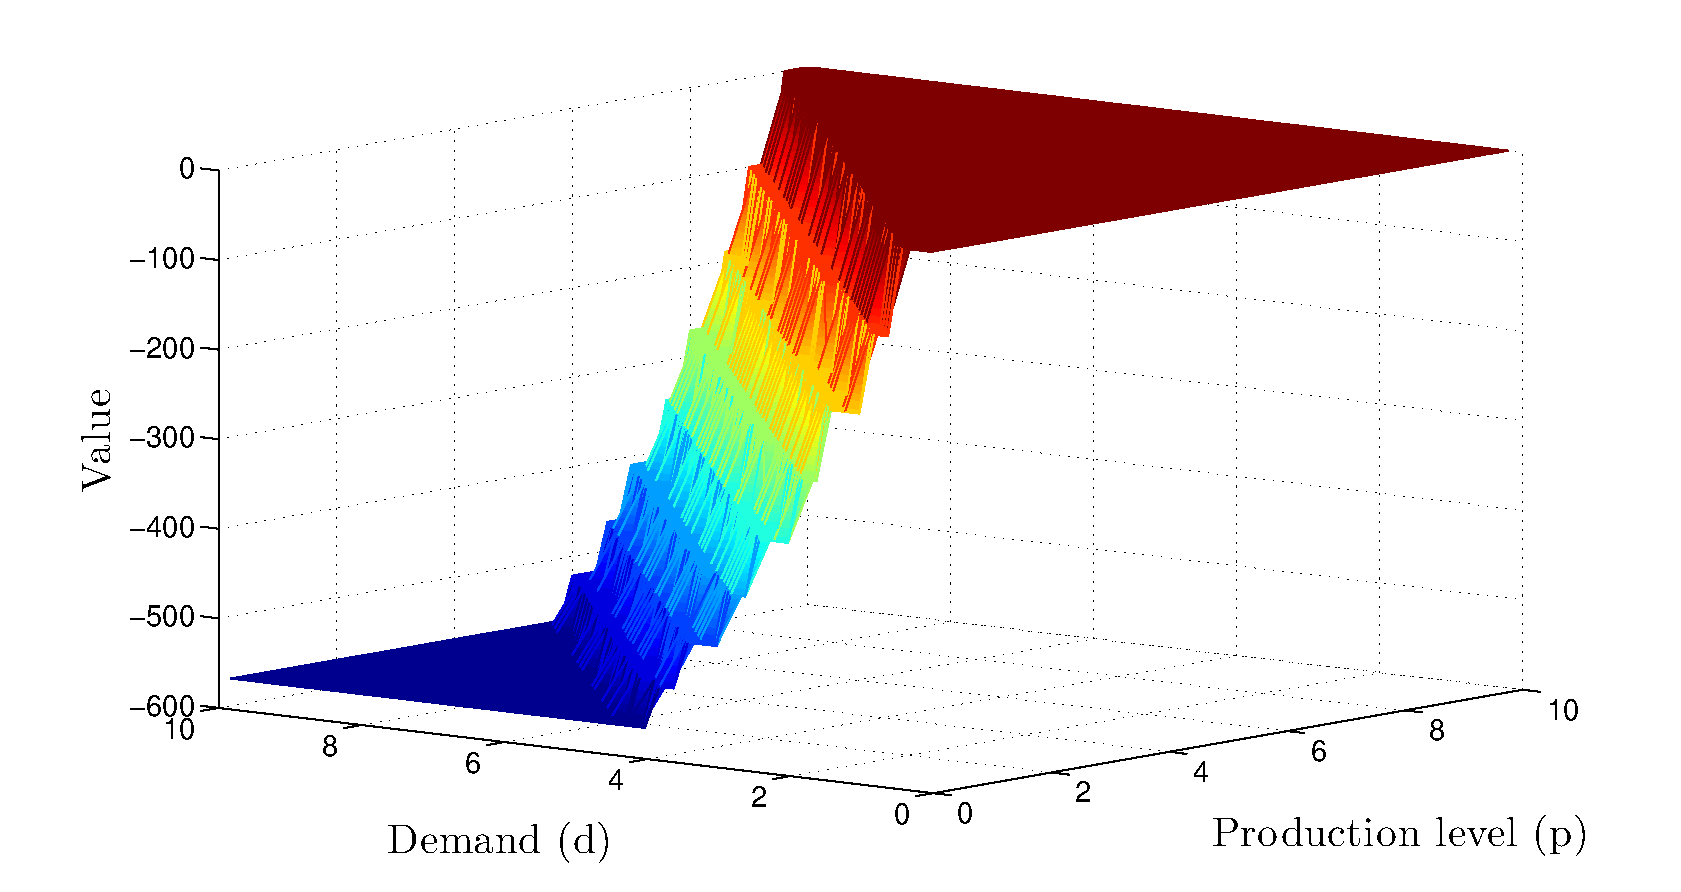
\includegraphics[width=250pt]{sep.pdf}
\vspace{-3mm}
\caption{The optimal value function for the robust energy production game at horizon 8. 
The increase and decrease variables where set to $dec_{prd} = inc_{prd} = 1.0$ and $dec_{nat} = inc_{nat} = 0.5$, respectively.}
\label{fig:sepvfunc}
\end{figure}

%%%%%%%%%%%%%%%%%%%%%%%%%%%%%%%%%

In Figure \ref{fig:sepvfunc} we show the optimal value function
for the robust energy production game at horizon 8. The value
function shows that the highest value is attained when the energy provided
exceeds demand. This is clearly evident given the nature of the reward structure.
When the demand exceeds the amount produced, the value is at its lowest.
Here we note that the value function decreases in a step-wise manner
from the point where where production level meets demand. This indicates
that production levels just beneath demand have a higher value than
those well below demand.
